\section{Thermal Expansion}
\label{sec:thermalExpansion}

\begin{frame}{Thermal Expansion Motivation}
  \begin{itemize}
    \item Strong feedback.
    \item Metallic fuels.
    \item Small active fuel region with high leakage ($\leakage \approx 20\%$).
    \item \gls{ebr-ii} designed and built by \gls{anl} \cite{PlentifulEnergy}.
      \begin{itemize}
        \item Full-power demonstrations from April 1986 \cite{ebriitests}.
        \item \gls{ulof}.
        \item \gls{ulohs}.
      \end{itemize}
  \end{itemize}
\end{frame}

\begin{frame}{Material Properties}
  \begin{figure}
    \centering
    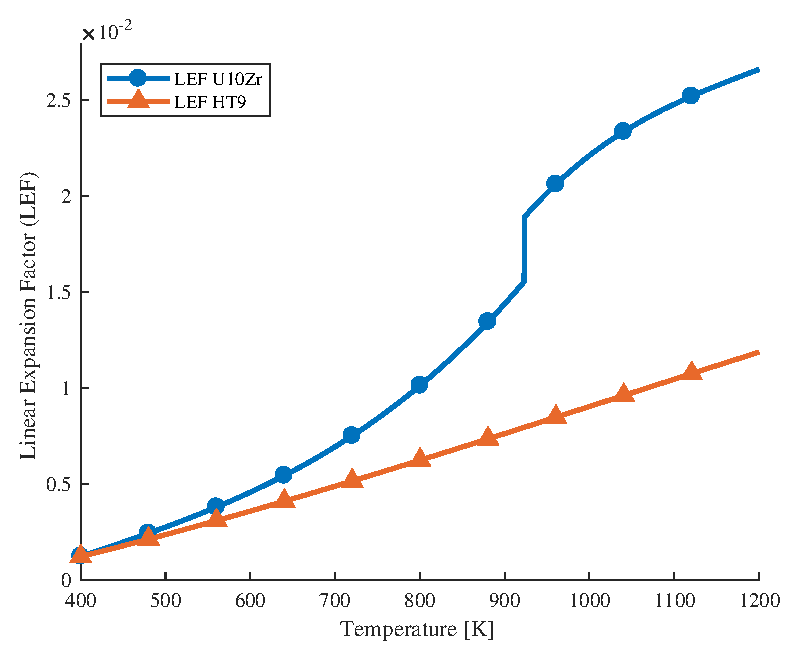
\includegraphics[width=0.7\textwidth]{lef_plot}
    \caption{Linear Expansion Factor for HT9 Steel and U10Zr Fuel.}
    \label{fig:lef_plot}
  \end{figure}
\end{frame}

\begin{frame}{Simplified Thermal Expansion Model}
  \begin{itemize}
    \item Leakage Effects.
      \begin{itemize}
        \item Finite Elements.
          \begin{itemize}
            \item Radial ($x$ and $y$) directions expanded as structural
              material, HT9 stainless steel.
            \item Axial ($z$) direction expanded as fuel material, U10Zr.
          \end{itemize}
        \item Area Fractions.
          \begin{itemize}
            \item Fuel radius, $R_F$, expanded as U10Zr.
            \item All other material expanded as HT9 stainless steel.
            \item Area fractions are used to homogenize cross sections.
          \end{itemize}
      \end{itemize}
    \item Density Effects.
      \begin{itemize}
        \item Material densities must decrease to conserve quantity of material
          with expanded dimensions.
        \item Cross sections decrease proportionally according to $\Sigma = N \,
          \sigma$.
      \end{itemize}
  \end{itemize}
\end{frame}

\begin{frame}{Finite Element Expansion}
\end{frame}

\begin{frame}{Area Fraction Expansion}
  \begin{figure}
    \centering
    \subfloat{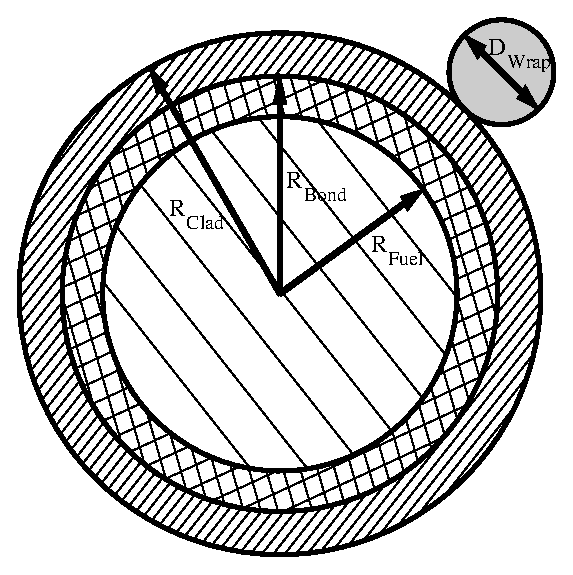
\includegraphics[width=0.35\textwidth]{pin_model}}
    \hspace{0.2in}
    \subfloat{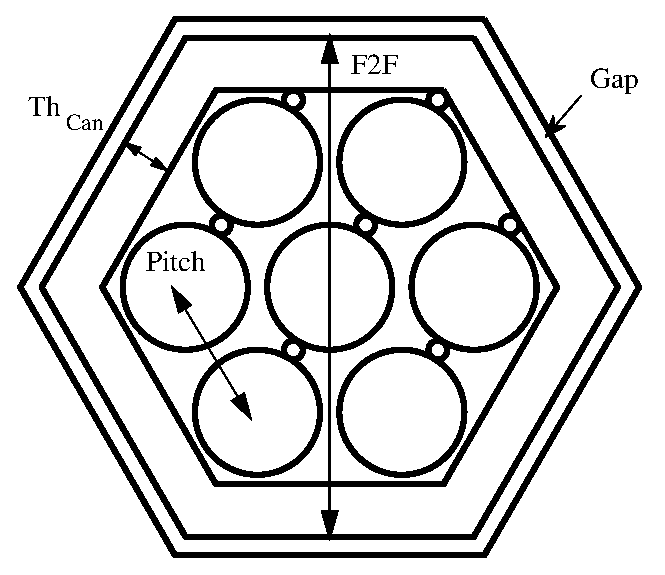
\includegraphics[width=0.35\textwidth]{hex_can}}
    \label{fig:assy_geometry}
  \end{figure}
\end{frame}

\begin{frame}{Conservation of Material \& Cross Section Effects}
\end{frame}

\begin{frame}{Volume Expansion}
  Given assumptions of uniform radial and axial expansion, volumes expand
  uniformly.
  \begin{align}
    \label{eq:volume_ratio}
    V^C &= \text{Cold Volume.}\\
    V^H &= \text{Hot Volume.}\\
    \frac{V^C}{V^H} &= \frac{1}{(F_r(\texpstruct))^2 (F_a(\texpfuel))}
  \end{align}
  \vspace{-0.1in}
  \begin{figure}
    \centering
    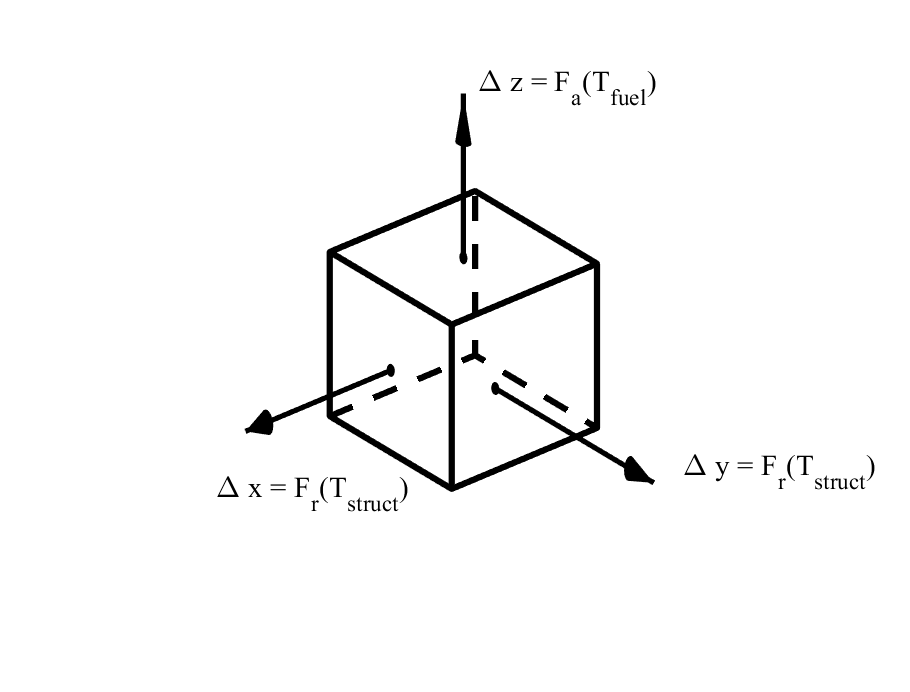
\includegraphics[width=0.7\textwidth]{thexp_figure}
    \label{fig:thexp_figure}
  \end{figure}
\end{frame}

\begin{frame}{Area Fraction Expansion}
  \begin{itemize}
    \item Area fraction expansion ratios are more difficult.
    \item $a_j^C$ and $a_j^H$ are calculated explicitly.
  \end{itemize}

  \begin{figure}
    \centering
    \subfloat{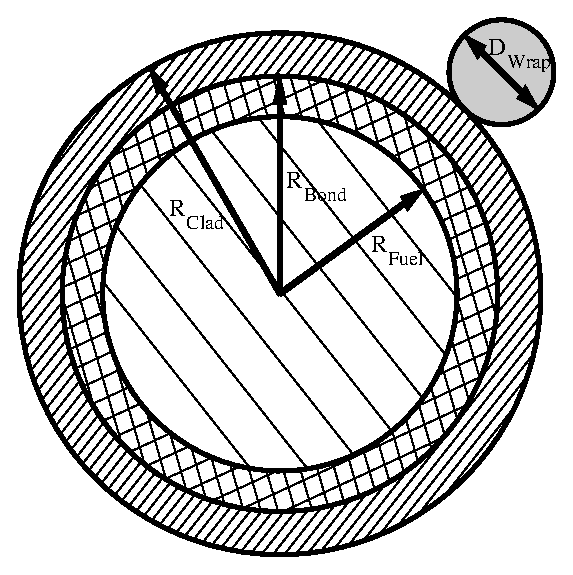
\includegraphics[width=0.35\textwidth]{pin_model}}
    \hspace{0.2in}
    \subfloat{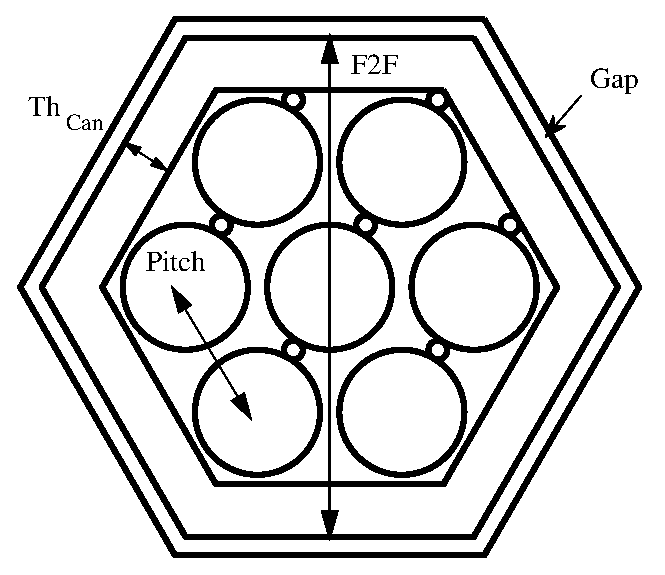
\includegraphics[width=0.35\textwidth]{hex_can}}
    \label{fig:assy_geometry}
  \end{figure}
\end{frame}

\begin{frame}{Number Density Expansion}
  \begin{itemize}
    \item The volume occupied by a material is the product of the 
      area fraction of the material and the volume of the element.
    \item To preserve the number of atoms in the reactor, the number density 
      must be diluted.
  \end{itemize}
  \begin{equation}
    \label{eq:nden_thexp_update}
    N_i^H = N_i^C \frac{a_j^C}{a_j^H} 
      \frac{1}{(F_r(\texpstruct))^2 (F_a(\texpfuel))}
  \end{equation}

  Then cross sections are proportional to number densities.
  \begin{equation}
    \Sigma = \sigma \, N
  \end{equation}
\end{frame}

\begin{frame}{Demonstration of Reactor Thermal Expansion}
  \begin{figure}
    \centering
    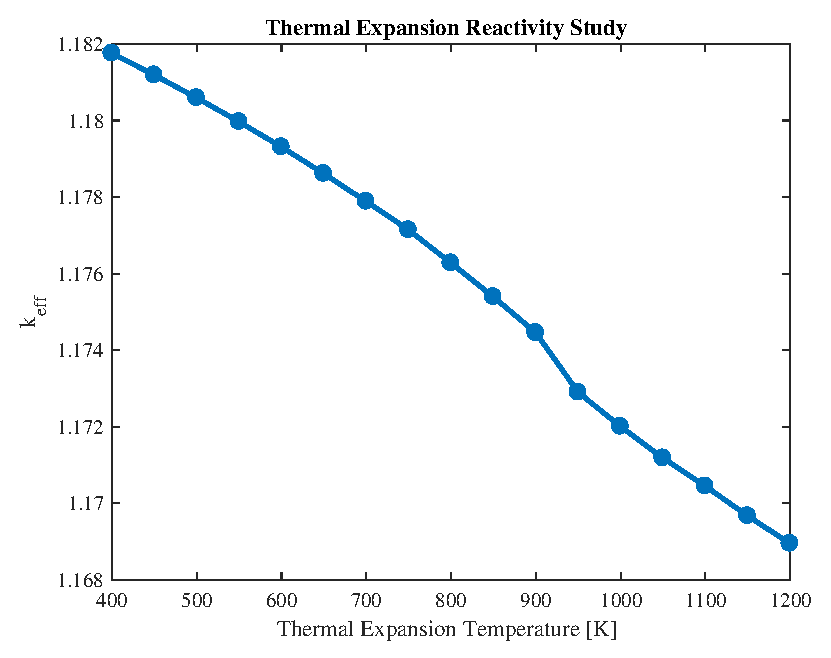
\includegraphics[width=0.7\textwidth]{thexp_study}
    \caption{Effective Neutron Multiplication Factor as a Function of 
      Thermal Expansion Temperature.}
    \label{fig:thexp_study}
  \end{figure}
  \begin{equation}
    \label{eq:reactivity_formula}
    \Delta \rho \units{\glsentryshort{pcm}} = \frac{\keff - \kref}{\keff \, \kref} \times
      10^5
  \end{equation}
\end{frame}
